%% LyX 1.6.5 created this file.  For more info, see http://www.lyx.org/.
%% Do not edit unless you really know what you are doing.
\documentclass[oneside,german,oneside]{scrbook}
\usepackage{ae,aecompl}
\usepackage[T1]{fontenc}
\usepackage[utf8]{inputenc}
\setcounter{secnumdepth}{3}
\setcounter{tocdepth}{3}
\usepackage{array}
\usepackage{url}
\usepackage{amstext}
\usepackage{graphicx}

\makeatletter

%%%%%%%%%%%%%%%%%%%%%%%%%%%%%% LyX specific LaTeX commands.
\providecommand{\LyX}{L\kern-.1667em\lower.25em\hbox{Y}\kern-.125emX\@}
%% Because html converters don't know tabularnewline
\providecommand{\tabularnewline}{\\}

\makeatother

\usepackage{babel}

\begin{document}

\title{Projektplan aidGer}


\author{Buchgraber (2512046), Gildein (2513744), Pirrung (2526016)\\
Gruppe 10}


\subject{- vertrauliches Dokument -}

\maketitle
\tableofcontents{}


\chapter{Einleitung\label{cha:Einleitung}}


\section{Zweck, Abgrenzung\label{sec:Zweck,-Abgrenzung}}

Seit März 2009 werden die Hilfskraftbeschäftigungen des Institutsverbund
der Informatik (IvI) von der Abteilung SE an der Universität Stuttgart
abgewickelt. Die Amtsübernahme stellte die Abteilung SE damals vor
große Herausforderungen: Man musste sich fachlich in die Thematik
einarbeiten, das bisherige Verfahren analysieren und daraus neue Geschäftsprozesse
etablieren. Hieraus entstand die Software mit dem Codename Hive, welche
die folgenden grundsätzlichen Hauptaufgaben zur Erleichterung der
täglichen Arbeiten zu erfüllen hat:
\begin{itemize}
\item Abwicklung der Arbeitsverträge (z.B. Einstellungen)
\item Genehmigungsvorlage und Panung der Finanzmittel
\item Berichtswesen und Controlling
\end{itemize}
Diese Softwarelösung hat jedoch einige Nachteile, die die Benutzung
nur eingeschränkt möglich macht. So sind beispielsweise die Geschäftsprozesse
nur auf Papier definiert und das Datenmodell gehört einer Überarbeitung
unterzogen. Darüber hinaus bildet die Lösung keine gesamte, homogene
Einheit, sondern besteht ferner aus einem inhomogenen Technologie-Mix,
der sich unter anderem aus einer OpenOffice-Anwendung, einem Ticket-System
und einem Unix Cron-Skript zusammensetzt.\\
\\
Dieser Zustand führt folglich zu immensen Schwächen bei der Effizienz
sowie der Benutzerfreundlichkeit der Software. Zudem wir die Abwicklung
von Geschäftsprozessen nur bedingt softwareseitig unterstützt.

Aus diesem Grund soll im Rahmen dieses Projekts eine Nachfolger-Software
entstehen, die den Namen aidGer tragen wird und bei der Abnahme Hive
schließlich ersetzen soll.


\subsection{Zweck des Projektplans}

Dieser Projektplan soll die Ziele des Projekts, die Zeitplanung für
deren Verwirklichung und alle relevanten Bedingungen für das Projekt
dokumentieren.

Die Planung des Projekts ist zu Anfang sehr schwierig, da die Informationen
über den Zeitaufwand für einzelne Teilaufgaben erst nach einer Einarbeitung
hinreichend genau geschätzt werden können. Deshalb wird der Plan im
Laufe des Projektes Änderungen erfahren, die vor allem die Zeitabläufe
betreffen können. 


\section{Projektüberblick, Motivation}

Im Rahmen des Projekts wird eine Desktop-Anwendung entwickelt, die
den Mitarbeitern der Abteilung SE die tägliche Arbeit bei der Verwaltung
der Hilfskraftbeschäftigungen des Institutsverbund der Informatik
erleichtern soll. Hierbei soll die Software auf das bestehende System
Hive aufbauen und dieses durch eine vollständige Neuentwicklung schließlich
ersetzen. Die zu entwickelnde Software trägt den Codenamen aidGer.\\
\\
aidGer soll sich der jetzigen Lösung in vielen Punkten ähneln,
wobei selbsterklärend die Schwächen und Nachteile von Hive (siehe
\ref{sec:Zweck,-Abgrenzung}) auszubessern sind, so dass im Endeffekt
ein einheitliches und produktiv einsetzbares Produkt entsteht.\\
\\
Die neue Software dient grundsätzlich zur Erleichterung der Erfassung
und Auswertung aller Prozesse, die bei der Verwaltung von Hilfskräften
anfallen.\\
\\
Zusammengefasst müssen die folgenden Vorgänge in aidGer unterstützt
werden:
\begin{itemize}
\item Stammdatenverwaltung
\item Budgetprüfung
\item Buchung von Beschäftigten
\item Controlling der Abrechnungen
\item Berichtswesen / Reporting
\item Vorgangserfassung
\end{itemize}
Hierzu wurde seither ein Ticket-System verwendet, welches hauptsächlich
die Funktion der Benachrichtigung von Hilfskräften via eMail übernimmt.
Dieses System soll mit aidGer weiterhin bestehen, wobei beide Systeme
möglichst als Einheit fungieren sollen.\\
\\
Damit die Software mit den bestehenden Daten weiterarbeiten kann,
wird eine Datenbankschnittstelle AdoHive parallel von einem externen
Team entwickelt, auf welche aidGer zu zugreifen hat.\\
\\
Zudem ist keine Authentifizierung beim Programmstart nötig.


\chapter{Formale Grundlagen\label{cha:Formale-Grundlagen}}


\section{Anforderungen an die Projektdurchführung}
\begin{itemize}
\item Der Auftraggeber ist die Abteilung SE der Universität Stuttgart.
\item Es handelt sich um ein unentgeltliches Projekt.
\item Das Projekt muss bis Mitte Juli auslieferbar sein.
\item Dabei wird es Ziel sein, das Projekt bis Ende Juni abzuschließen,
damit notfalls der Zeitpuffer von 2 Wochen für abschließende Arbeiten
genutzt werden kann.
\item Das Projekt soll in Java geschrieben werden, Version: Java SE 1.6.
\item Die Benutzeroberfläche soll mittels Java Swing gestaltet werden.
\end{itemize}

\section{Anforderungen an das Produkt}
\begin{itemize}
\item Moderne und intuitiv bedienbare Desktop-Anwendung
\item Erfassung aller Geschäftsvorgänge, die getätigt werden
\item Kompatibilität zur Datenbankschnittstelle AdoHive
\item Gute Benutzerfreundlichkeit
\item Übersichtliche und zeitgemäße Benutzeroberfläche
\item Kurze Einarbeitungszeit in das Programm
\item Plattformunabhängigkeit
\item Mehrsprachigkeit
\item Erweiterbarkeit
\item Gute Wartbarkeit
\end{itemize}

\section{Anforderungen an die Konformität mit Normen}

Da die Software auf das bestehende System Hive aufbauen soll, sollte
bei der Entwicklung darauf geachtet werden, dass aidGer diesem ähnelt
und jeder, der zuvor am alten System gearbeitet hat, nach kurzer Einarbeitungszeit
aidGer bedienen kann. Daher soll aidGer ein ähnliches Look\&Feel wie
seither erhalten. Darüber hinaus sollen die exportierte Berichte dem
Aussehen ähnlich wie den jetzigen entsprechen.\\
\\
Es müssen ferner Normen eingehalten werden, dass die Möglichkeit
des Fallbacks zum alten System Hive immer bestehen bleibt.


\section{Gesetzliche Auflagen}
\begin{itemize}
\item Schutz personenbezogener Daten vor Missbrauch, insbesondere keine
Weitergabe der Daten an Dritten%
\footnote{gemäß Bundesdatenschutzgesetz (BDSG)%
}.
\item Die entstehende Software ist ein urheberrechtlich geschütztes Werk
%
\footnote{gemäß Gesetz über Urheberrecht und verwandte Schutzrechte (UrhG)%
}.
\end{itemize}

\chapter{Leistungen der Vertragspartner\label{cha:Leistungen-der-Vertragspartner}}


\section{Lieferumfang}

Folgende Resultate werden dem Auftraggeber ausgeliefert:
\begin{itemize}
\item Java-Anwendung
\item Quellcode
\item Benutzerhandbuch
\item Installationsanleitung
\item Spezifikation und andere benötigte Dokumente nach Anfrage
\end{itemize}

\section{Resultate, die nicht zum Lieferumfang gehören}

Der Kunde kann alle Resultate bzw. Dokumente nach Anfrage erhalten,
mit Ausnahme von:
\begin{itemize}
\item streng vertraulich oder vertraulich gekennzeichnete Dokumente und
\item Zwischendokumente.
\end{itemize}

\section{Leistungen des Auftragsgebers (Beistellungen)}

Der Auftraggeber
\begin{itemize}
\item stellt den Server, auf welchem aidGer installiert wird, selbst zur
Vefügung.\\
Dieser muss den folgenden Voraussetzungen genügen:

\begin{itemize}
\item Prozessor: 300 MHz, Arbeitsspeicher: 1024 MB, Festplatte: 512 MB
\item Java Virtual Machine (JVM) der Version 1.6 installiert
\item Datenbankschnittstelle AdoHive und zugehöriges Datenbankmodell installiert
\item bisheriges Ticket-System installiert
\end{itemize}
\item ist für die Sicherungskopien der Daten selbst verantwortlich.
\item stellt das derzeitige System Hive bereit.
\item steht für weitere Fragen zur Verfügung.
\end{itemize}

\section{Externe Meilensteine\label{sec:Externe-Meilensteine}}

Folgende Ergebnisse sollen an den angegebenen Terminen an den Kunden
ausgeliefert werden (siehe \ref{sec:Terminplan}):

\begin{center}
\begin{tabular}{|c|l|c|}
\hline 
\textbf{ID} & \textbf{Externer Meilenstein} & \textbf{Termin}\tabularnewline
\hline
\hline 
M1 & UI-Prototyp & 09.03.2010\tabularnewline
\hline 
M2 & Spezifikation & 23.03.2010\tabularnewline
\hline 
M3 & Entwurf & 13.04.2010\tabularnewline
\hline 
M4 & Release Candidate & 29.06.2010\tabularnewline
\hline 
M5 & Endabnahme & 14.07.2010\tabularnewline
\hline
\end{tabular}
\par\end{center}


\section{Abnahmeprozedur}

Das Produkt wird dem Kunde mit obigen Lieferumfang ausgeliefert. Die
Installation und die Wartung übernimmt der Kunde dann selbst.

Unter Umständen sind Nachverhandlungen möglich, so dass der Support
und die Weiterentwicklung an aidGer entgeltlich weitergeführt wird.


\section{Änderungsverfahren}

Nach Auslieferung ist es die Aufgabe des Kunden, gewünschte Änderungen
an der Software vorzunehmen (Wartungszuständigkeit des Auftraggebers).
Änderungen, welche vor der Auslieferung bekannt gegeben werden, können
mit eventueller Verzögerung der Auslieferung vorgenommen werden. Außerdem
kann ein Änderungswunsch abgelehnt werden, falls dieser den Zeitaufwand
immens steigern würde und somit den Auslieferungstermin gefährden
könnte.


\chapter{Richtlinien für die Entwicklung\label{cha:Richtlinien-f=0000FCr-die}}


\section{Konfigurationsmanagement}

Als Konfigurationsmanagement muss das Werkzeug \textit{Git} von allen
eingesetzt werden.\\
\\
Dabei müssen die folgende Artefakte via Konfigurationsmanagement
verwaltet werden:
\begin{itemize}
\item Analysenotizen, Projektplan
\item Anforderungsspezifikation
\item Systementwurf
\item Quellcode
\item Benutzerhandbuch und Installationsvorschrift
\item Review-Berichte
\item Testpläne
\item Zeitaufwand der Mitarbeiter
\end{itemize}
Geprüfte und abgenommene Dokumente könnern nur nach Absprache mit
dem Kunde bzw. dem Bearbeiter geändert werden. Anschließend müssen
geänderte Dokumente erneut geprüft werden.\\
\\
Zudem muss ein hierarchisches Bezeichnungsschema verwendet werden.


\section{Design- und Programmier-Richtlinien\label{sec:Design--und-Programmier-Richtlinien}}
\begin{itemize}
\item Die Projektsprache ist Deutsch.
\item Codekommentare müssen in Englisch verfasst werden und in reichlicher
Zahl vorhanden sein.
\item Die Software muss vollständig in der Programmiersprache Java geschrieben
werden.
\item Alle Programmierer müssen sich an die \textit{Code Conventions for
the Java Programming Language}%
\footnote{http://java.sun.com/docs/codeconv/%
} halten.
\item Alle Dokumente müssen mit \LaTeX \, oder \LyX{} geschrieben werden.
\end{itemize}

\section{Einsatz von Werkzeugen\label{sec:Einsatz-von-Werkzeugen}}
\begin{itemize}
\item IDE: Eclipse 3.5.1 mit dem UML-Plugin SDE for Eclipse 5.2 (Visual
Paradigm)
\item Externe Bibliothek für den PDF-Export: iText 5.0.1
\item Konfigurationsmanagement: Git 1.6
\item Projektmanagement: Redmine 0.9.2
\item Aufwandserfassung und -auswertung: Fred 1.4
\item Review-Organisation: RevAger 1.2
\item Testüberdeckung: CodeCover 1.0
\item Testfallverwaltung: Justus 1.0
\item Dokumentation: \LaTeX $\text{ }2_{\epsilon}$ und \LyX{} 1.6.5
\end{itemize}

\chapter{Entwicklungsprozess\label{cha:Entwicklungsprozess}}


\section{Strategie für die Entwicklung und Integration}

Um eine hohe Qualität der Resultate und die Einhaltung der Ablaufplanung
zu garantieren, müssen bei der Entwicklung der Software ingenieursmäßige
Prinzipien eingesetzt werden. So werden alle während der Entwicklung
entstehende Artefakte wie beispielsweise die Spezifikation und das
Benutzerhandbuch einem Review unterzogen und zusätzlich getestet.\\
\\
Eine gute und vor allem aktuelle Dokumentation aller Arbeitsergebnisse
ist essentiell, um die Verwendung dieser Dokumente durch Dritte zu
ermöglichen.\\
\\
Darüber hinaus müssen die festgelegten Programmierrichtlinien (siehe
\ref{sec:Design--und-Programmier-Richtlinien}) eingehalten werden,
um eine hohe Qualität des Programmcodes sicherzustellen.


\section{Qualitätssicherung}

Die Qualitätssicherung soll eine hohe Qualität des Entwicklungsprozesses
und der erzielten Ergebnisse sicherstellen. Das erfordert, dass die
angestrebten Qualitätsaspekte dokumentiert und Vorgehensweisen entwickelt
werden.\\
\\
\textit{Organisatorische Maßnahmen:} Die Fortschritte werden alle
zwei Wochen geprüft und unter Umständen die Zeitplanung entsprechend
angepasst.\\
\\
\textit{Analytische Maßnahmen:} Die Dokumente werden in Reviews
geprüft und das Programm einem Test nach einem erstellten Testplan
unterzogen. Abgenommene Dokumente stellen Meilensteine dar, auf welche
dann aufgebaut werden kann.


\section{Phasen der Entwicklung}

Das Projekt umfasst die folgenden sechs Phasen:
\begin{itemize}
\item Analyse
\item Spezifikation der Anforderungen
\item Architekturentwurf
\item Codierung
\item Test
\item Abnahme
\end{itemize}

\section{Dokumentationsplan}

Es werden folgende Dokumente während der Entwicklung entstehen:
\begin{itemize}
\item Fragenkatalog für die Kundenbefragung
\item Analysenotizen, Projektplan
\item Spezifikation
\item Entwurf
\item Benutzerhandbuch
\item Testplan zum Test des Systems mit den zugehörigen Testdaten sowie
das Testprotokoll
\item Review-Berichte
\end{itemize}
Die Richtlinien für Dokumente in diesem Plan gelten für alle entstehenden
Dokumente.


\section{Prüfungen (Reviews und Tests)}

Folgende Resultate müssen einer Prüfung unterzogen werden:
\begin{itemize}
\item Spezifikation
\item Benutzerhandbuch
\item Entwurf
\item Codierung
\end{itemize}
Die Durchführung von Reviews unterliegen folgenden Richtlinien:
\begin{itemize}
\item Formale Reviews mit einem Moderator, 2-3 Gutachtern und einem Autor.
\item Die Review-Dauer ist auf 2 Stunden beschränkt.
\end{itemize}
Folgende Tests müssen durchgeführt werden:
\begin{itemize}
\item Modultest der einzelnen Komponenten
\item Systemtest der gesamten Software
\item Abnahmetest zusammen mit dem Kunden
\end{itemize}

\chapter{Anforderungen an die Umgebung\label{cha:Anforderungen-an-die}}


\section{Infrastruktur (Büros, Rechnersysteme, Software)}

Folgendes muss vom Auftragnehmer bereitgestellt werden:
\begin{itemize}
\item Es müssen mindestens 3 Rechner zur Verfügung stehen, auf denen alle
eingesetzen Werkzeuge lauffähig sind (siehe hierzu \ref{sec:Einsatz-von-Werkzeugen}).
\item Zentraler Server für die Projektablage, das Projektmanagement sowie
das Konfigurationsmanagement.
\item Verfügbarkeit von Rechnern mit Linux, Windows und Mac OS.
\item Internetpräsenz des Projekts aidGer%
\footnote{http://www.aidger.de%
}
\end{itemize}

\section{Leistungen Dritter im Unternehmen}

Alle Mitarbeiter im Unternehmen sind an diesem Projekt beteiligt.


\section{Leistungen externer Lieferanten}

Das externe Entwicklungsteam AdoHive muss die Datenbankschnittstelle
AdoHive pünktlich an uns liefern. Es besteht ferner keine vertragliche
Beziehung zu diesem externen Lieferant (siehe \ref{sec:Risiken-und-ihre}).


\chapter{Projektorganisation\label{cha:Projektorganisation}}


\section{Schnittstelle zum Auftraggeber}

Die Vertretung zum Kunde übernimmt der Mitarbeiter Christian Buchgraber.


\section{Schnittstelle zur Aufbauorganisation}

Diese Schnittstelle übernimmt der Mitarbeiter Philipp Pirrung.


\section{Schnittstelle zu anderen Projekten}

Es wird keine Schnittstelle benötigt, da keine andere Projekte im
Unternehmen existieren.


\section{Schlüsselpersonen}

\begin{tabular}{l>{\raggedright}p{6in}}
\textbf{Kunde:} & Herr Daniel Kulesz\\
eMail: \url{daniel.kulesz@informatik.uni-stuttgart.de}\tabularnewline
\noalign{\vskip0.4cm}
\textbf{Betreuer:} & Herr Ivan Bogicevic\\
eMail: \url{ivan.bogicevic@informatik.uni-stuttgart.de}\tabularnewline
\noalign{\vskip0.4cm}
\textbf{Projektleiter:} & Herr Philipp Gildein\\
eMail: \url{gildeipp@studi.informatik.uni-stuttgart.de}\tabularnewline
\noalign{\vskip0.4cm}
\textbf{Mitarbeiter 1: } & Herr Phlipp Pirrung\\
eMail: \url{pirrunpp@studi.informatik.uni-stuttgart.de}\tabularnewline
\noalign{\vskip0.4cm}
\textbf{Mitarbeiter 2:} & Herr Christian Buchgraber\\
eMail: \url{buchgrcn@studi.informatik.uni-stuttgart.de}\tabularnewline
\noalign{\vskip0.4cm}
\end{tabular}


\section{Berichtswesen}

Jeder Mitarbeiter ist verpflichtet, seinem direkten Vorgesetzten Bericht
zu erstatten. Im Falle des Projektleiters ist der direkte Vorgesetzte
der Manager des Unternehmens. Der Projektleiter ist der direkte Vorgesetzte
aller übrigen Mitarbeiter.


\chapter{Entwicklungsplan\label{cha:Entwicklungsplan}}


\section{Projektstrukturplan (Arbeitsgliederung)}

Das Projekt umfasst folgende Arbeitspakete:
\begin{itemize}
\item Analyse: Befragen des Kunden zur Erhebung des Ist- und Soll-Zustands
\item Projektplanung: Festlegen der einzelnen Arbeitspakete und Meilensteine,
Terminplanung
\item Einarbeiten in die Thematik
\item Spezifikation: Festlegen der Anforderungen an die Funktionalität des
Systems, Festlegen der nicht-funktionalen Anforderungen
\item Durchführen eines Spezifikationsreviews
\item Nachbearbeiten der Spezifikation
\item Erstellen eines Benutzerhandbuchs
\item Erstellen eines Entwurfs: Festlegen der Systemarchitektur
\item Durchführen eines Entwurfsreviews
\item Nachbearbeiten des Entwurfs
\item Implementieren des Programms in Java
\item Erstellen eines Testplans
\item Durchführen des Modultests
\item Korrektur des Modultests
\item Durchführen des Systemtests
\item Korrektur des Systemtests
\item Korrigieren des Programms und Überarbeitung der erstellten Dokumente
\item Ausliefern eines Release Candidates an den Kunden
\item Ausliefern an den Kunden
\end{itemize}

\section{Terminplan\label{sec:Terminplan}}

\begin{flushleft}
Der Terminplan ist als Gantt-Diagramm graphisch dargestellt:
\par\end{flushleft}

\begin{center}
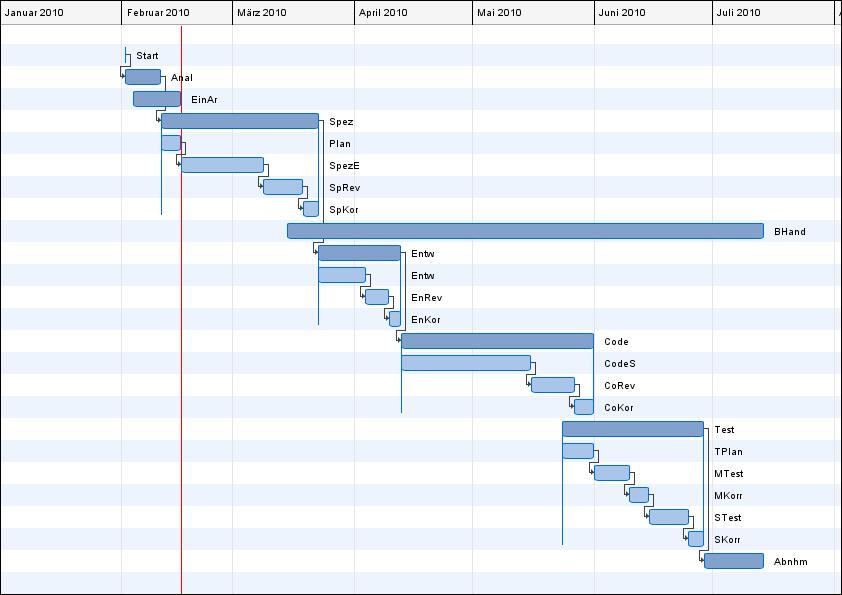
\includegraphics[width=1\textwidth]{gantt}
\par\end{center}

\begin{flushleft}
Folgende nicht eindeutige Abkürzungen wurden verwendet:
\par\end{flushleft}
\begin{itemize}
\item Anal - Erstellung der Analyse
\item EinAr - Einarbeitung in die Thematik
\item SpRev - Review der Spezifikation
\item SpKor - Korrektur der Spezifikation
\item BHand - Benutzerhandbuch
\item TPlan - Erstellung eines Testplans
\item CoKor - Korrektur des Programms
\item MTest - Modultest
\item STest - Systemtest
\item Abnhm - Abnahme durch den Kunde
\end{itemize}

\section{Risiken und ihre Bewertung\label{sec:Risiken-und-ihre}}

Da der Erfolg des Projekt stark am externen Lieferant AdoHive abhängt,
muss folglich gesichert sein, dass die Datenbankschnittstelle rechtzeitig
und einsatzfähig von dem genannten Entwicklungsteam ausgeliefert wird.
Da keine Vertragsbeziehungen zwischen dem externen Lieferant und unserem
Unternehmen bestehen, kann rechtlich gesehen ein Schadenersatzanspruch
nicht geltend gemacht werden. Es kann jedoch angenommen werden, dass
dieser Umstand mit geringer Wahrscheinlichkeit eintritt, da sich das
Entwicklungsteam aus Mitarbeitern der Abteilung SE zusammensetzt,
die ein begründetes Interesse am Erfolg des Projekts haben. Sollte
dieser Fall aber trotz allem eintreten, so muss das entstandene Risiko
als äußert kritisch eingestuft werden, da unter Umständen die Software
aufgrund der zwingenden Abhängigkeit zur Datenbankschnittstelle nicht
ausgeliefert werden kann.\\
\\
Nicht alle Mitarbeiter im Team haben bislang an Java-Projekten
mit vergleichsbarem Umfang teilgenommen. Dieses Risiko tritt immer
ein und kann als unkritisch eingestuft werden. Die Gegenmaßnahme besteht
darin, dass unerfahrenen Mitarbeiter an einer mehrtägigen Java-Schulung
teilnehmen, wobei die dadurch entstandenen Kosten vom Unternehmen
gedeckt werden.\\
\\
Ferner ist zu berücksichtigen, dass sich in einigen Projektphasen
die Mitarbeiter aufgrund von Prüfungsvorbereitungen nicht vollzeitig
mit der Softwareentwicklung befassen können. So könnte es im Extremfall
zu Lieferverzögerungen der Meilensteine kommen. Dieses Risiko tritt
mit mittlerer Wahrscheinlichkeit ein. Um dies zu vermeiden, ist eine
gute Projektplanung und ein gutes Zeitmanagement von jedem Mitarbeiter
zwingend verlangt.


\chapter{Anhang\label{cha:Anhang}}


\section{Versionshistorie}


\subsubsection*{Version 0.2.1 (19.02.2010)}
\begin{itemize}
\item Berichtigung der Betreuerangabe
\item Angabe der einzusetzenden Bibliotheken hinzugefügt
\item Vermerk der Internetpräsenz des Projekts ergänzt
\item Verweis auf die \textit{Java Code Conventions} hinzugefügt
\end{itemize}

\subsubsection*{Version 0.2 (18.02.2010)}
\begin{itemize}
\item Erstellung des Kapitels \ref{cha:Anhang}
\item Fehlende Betreuerangaben hinzugefügt
\item Liste der Leistungen seitens des Auftragsgebers ergänzt
\item Liste der Anforderungen an das Produkt gekürzt
\end{itemize}

\subsubsection*{Version 0.1.2 (16.02.2010)}
\begin{itemize}
\item Korrekturen und Ergänzungen in allen Kapiteln vorgenommen
\end{itemize}

\subsubsection*{Version 0.1.1 (15.02.2010)}
\begin{itemize}
\item Erstellung der Kapitel \ref{cha:Entwicklungsprozess}, \ref{cha:Projektorganisation}
und \ref{cha:Entwicklungsplan}
\end{itemize}

\subsubsection*{Version 0.1 (14.02.2010)}
\begin{itemize}
\item Erstellung der Kapitel \ref{cha:Einleitung}, \ref{cha:Formale-Grundlagen},
\ref{cha:Leistungen-der-Vertragspartner}, \ref{cha:Richtlinien-f=0000FCr-die}
und \ref{cha:Anforderungen-an-die}
\end{itemize}

\end{document}
